%!TEX root = ../../../adrien_gomar_phd.tex

Two algorithms that automatically choose the time instances in order to
minimize the condition number are presented: first, the Almost
Periodic Fourier Transform (APFT) algorithm, initially proposed in the
literature for electronics problems and implemented by
\citet{ThesisGuedeney} in his PhD thesis, is described, then a gradient-based
optimization algorithm over the condition number (OPT), developed in
the current PhD work, is presented.

\subsection{Almost-Periodic Fourier Transform algorithm (APFT)}
\label{sec:apft_algorithm}
Based on the work of \citet{Kundert1988} in
electronics, the APFT
algorithm has been implemented by \citet{ThesisGuedeney} 
during his PhD thesis. The algorithm is designed
to maximize the orthogonality of the multi-frequential
IDFT matrix in order to minimize its condition number. To do so, a
Gram-Schmidt orthogonalization procedure is conducted.  First, the period 
associated with the smallest frequency ($2 \pi / \omega_{min}$) 
is oversampled with $M$ evenly spaced time
instances, $M\gg2N+1$ being specified by the user with $N$ the number of
frequencies. Considering these time instances, a rectangular
multi-frequential IDFT matrix is built. This rectangular matrix can be seen
as a set of $M$ vectors of length $2N+1$.
The first vector noted $V_0$ (corresponding
to $t=0$) is arbitrarily chosen as the first time instance and any
component in the direction of $V_0$ is removed from the following
vectors using the Gram-Schmidt formula:
\begin{equation}
   V_s = V_s - \frac{V_0^\top V_s}{V_0^\top V_0} V_0, \quad s=1 \cdots M-1.
   \label{GramSchmidtAlgo}
\end{equation}
The remaining vectors are now orthogonal to $V_0$. 
Initially, the vectors had the same Euclidean norm.
Therefore, the vector that has now the largest norm is
the most orthogonal to $V_0$.
It is thus assigned to $V_1$. The previous
operations are then performed on the $M-2$ remaining vectors using $V_1$
as starting point. This process is repeated until the required $2N+1$ vectors
are defined. As a time instance corresponds to a vector, $2N+1$ time instances are obtained, 
which enables the construction of the multi-frequential
IDFT matrix. This algorithm is summarized in
Algo.~\ref{alg:algo_APFT}.

\begin{algorithm}
\caption{The Almost Periodic Fourier Transform Algorithm (APFT)}
\label{alg:algo_APFT}
\begin{algorithmic}
\STATE $\omega_{min} \leftarrow min \left( |\omega_k |,\quad 1 \leqslant k \leqslant N \right)$
\FOR{$m \leftarrow 0 \cdots M-1$}
    \STATE $t_m \leftarrow \displaystyle\frac{2\pi}{\omega_{min}}\frac{m}{M}$
\ENDFOR
\FOR{$n \leftarrow 1 \cdots 2N$}
   \FOR{$m \leftarrow n+1 \cdots M$}
  \STATE $ V_{m} \leftarrow V_{m} - \displaystyle\frac{V_{n}^\top \cdot V_{m}}{V_{n}^\top \cdot V_{n}} V_{n}$
   \ENDFOR
   \STATE \textbf{argmax()} returns the index of the largest member of a set
   \STATE $k=\textbf{argmax} \left( \| V_s^n \|,\quad n+1\leqslant s \leqslant M\right) $
   \STATE $\textbf{swap}(V_{n+1},V_{k})$
   \STATE $\textbf{swap}(t_{n+1},t_{k})$
\ENDFOR
\STATE $\mathbb{T}_{optimized} \leftarrow [t_0 \cdots t_{2N}]$
\end{algorithmic}
\end{algorithm}

\subsection{Gradient-based optimization algorithm (OPT)}
\label{sec:algo_opt}
A more direct approach is to seek directly a set of time instances
that minimize the condition number of the associated multi-frequential IDFT matrix. 
This minimization problem can be solved numerically by an optimization algorithm.

The limited memory optimization method of
\citet{Byrd1995} (noted L-BFGS-B) is
used to look for a minimum of the condition number of the
multi-frequential IDFT matrix $\kappa \left(E^{-1} \left[\mathbb{T} \right]
\right)$ as function of the time instances vector $\mathbb{T}$. This
quasi-Newton algorithm approximates the inverse Hessian matrix
$H(\kappa \left(E^{-1} \left[\mathbb{T} \right] \right))^{-1}$ with the
BFGS formula in order to decrease the objective $\kappa \left(E^{-1}
  \left[\mathbb{T} \right] \right)$ in the direction $-H(\kappa
\left(E^{-1} \left[\mathbb{T} \right] \right))^{-1}\nabla \kappa \left(E^{-1}
  \left[\mathbb{T} \right] \right)$. In the present case, the
derivative $\nabla \kappa \left(E^{-1} \left[\mathbb{T} \right] \right)$ of
the objective with respect to the time instances is approximated by
a first-order finite differences. The descent direction is
associated with the search for a zero of the gradient, which is a
necessary condition for an extrema, in a second-order Taylor series.
Finally, a line search on $\alpha$ is performed to minimize $\kappa
\left(E^{-1} \left[\mathbb{T} - \alpha H(\kappa \left(E^{-1} \left[\mathbb{T}
      \right] \right))^{-1} \nabla \kappa \left(E^{-1} \left[\mathbb{T}
      \right] \right) \right] \right)$.  An open-source implementation of this
broadly-used algorithm is
employed~\cite{Nocedal1980}.

Gradient descent methods being local, the L-BFGS-B method converges to a local
minimum of the condition number. This minimum is unsatisfying if the
starting time instances vector $\mathbb{T}$ is not well chosen, therefore a strategy
to find an appropriate initial point is required. To this aim, the smallest
angular frequency $\omega_{min}$ is used as a base angular frequency to create a set $\Omega$:
\begin{equation}
    \Omega = [\frac{1}{M} \omega_{min} \cdots \frac{m+1}{M} \omega_{min} \cdots \omega_{min}],
    \label{eq:slitted_period}
\end{equation}
where $M$ denotes the desired number of initial guesses.
This gives a set of periods. Each of them are then evenly sampled to obtain a
set of time instances $\mathbb{T}_m$:
\begin{equation}
    \mathbb{T}_m = \left[ 0, \frac{2 \pi M}{ (2N + 1) (m+1) \omega_{min}} \cdots 
                             \frac{2N \pi M}{ (2N + 1) (m+1) \omega_{min}} \right]
    \label{eq:set_of_tlv}
\end{equation}
These time instances sets are finally used as initial guesses for the
L-BFGS-B algorithm.

The multi-frequential IDFT matrix is then built for
each of these time instances and the corresponding condition numbers are
computed. A large number $M$, typically thousands, of fractions of the
greatest period gives a large set of potential time instances vectors.
This is acceptable given the very low cost of the computation of the
condition number on such small matrices of size $(2N + 1) \times
(2N+1)$.  From this set, the time instances vector associated with the
multi-frequential IDFT matrix having the smallest condition number is
taken as a starting point.  The optimization algorithm actually achieves
a local adjustment of the time instances.

In this way, the exploitation capability of the gradient-based
optimizer is well combined with the exploration capacity of the
sampling. The OPT algorithm is summarized in Algo.~\ref{alg:algo_opt}.
\begin{algorithm}
\caption{The gradient-based optimization algorithm (OPT)}
\label{alg:algo_opt}
\begin{algorithmic}
\STATE $\omega_{min} \leftarrow min \left( |\omega_k |,\quad 1 \leqslant k \leqslant N \right)$
\FOR{$m \leftarrow 0 \cdots M - 1$}
    \STATE $\omega_m \leftarrow \frac{m + 1}{M} \cdot \omega_{min}$
    \FOR{$i \leftarrow 0 \cdots 2N$}
        \STATE $t_i \leftarrow \displaystyle\frac{i \cdot 2 \pi}{\omega_m \cdot (2N + 1)}$
    \ENDFOR
    \STATE $\mathbb{T}_m \leftarrow [t_0 \cdots  t_i \cdots t_{2N}]$
    \STATE $C_m \leftarrow \kappa \left(E^{-1} \left[\mathbb{T}_m \right] \right)$
\ENDFOR
\STATE \textbf{argmin()} returns the index of the smallest member of a set
\STATE $k \leftarrow \textbf{argmin}\left(C_m,\quad 0\leqslant m \leqslant M-1\right)$
\STATE $\textbf{min\_l-bfgs-b}\left(\kappa \left(E^{-1} \left[\mathbb{T}\right]\right), \mathbb{T}_{ini}\right)$ returns the optimal 
time instances vector $\mathbb{T}$ using the condition number $\kappa\left(E^{-1} \left[\mathbb{T}\right]\right)$ as objective function 
for the L-BFGS-B algorithm and  $\mathbb{T}_{ini}$ as starting point.
\STATE $\mathbb{T}_{optimized} \leftarrow 
  \textbf{min\_l-bfgs-b}\left(\kappa\left(E^{-1} \left[\mathbb{T}\right]\right), \mathbb{T}_{ini}=\mathbb{T}_k\right)$
\end{algorithmic}
\end{algorithm}

\subsection{Assessment of the algorithms}
Taking the same independent couple of frequencies $(f_1, f_2)$ as the one
used is Sec.~\ref{sec:condition_cror_ael}, the condition number of the
multi-frequential DFT matrix $\kappa (E)$ is computed, highlighting
the ability of the different algorithms to choose the time instances that
minimize the condition number, for any input frequencies. This
assessment is only made for two frequencies, but the results are similar
when increasing the number of frequencies. As two frequencies are
involved, five time instances are required. The results for the three
algorithms are depicted in Fig.~\ref{fig:bench_algo}: (i)~APFT: the
Almost Periodic Fourier Transform algorithm, (ii)~OPT: the
gradient-based OPTimization algorithm and (iii)~EVE: EVEnly spaced
time instances oversampling the largest period as done in
\citet{Gopinath2007} using $2N+1$ time
instances and in \citet{Ekici2007} and \citet{Ekici2008} using $3N+1$
time instances.
Table~\ref{tab:algo_sum} gives some statistics about the results obtained
with each algorithm to give the reader a quantitative overview of the
efficiency of the different algorithms.
\begin{figure}[htp]
  \centering 
    \subfigure[EVE $(2N + 1)$]{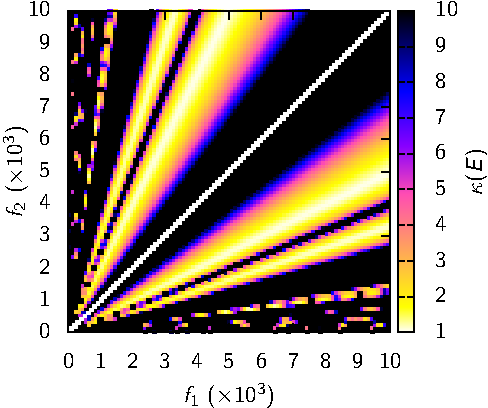
\includegraphics[width=.45\textwidth]{algo_equi_assessment.pdf}}
    \subfigure[EVE $(3N + 1)$]{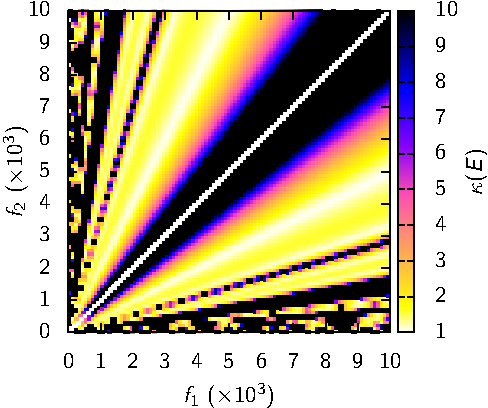
\includegraphics[width=.45\textwidth]{algo_equi_3n_assessment.pdf}}
    \subfigure[APFT]{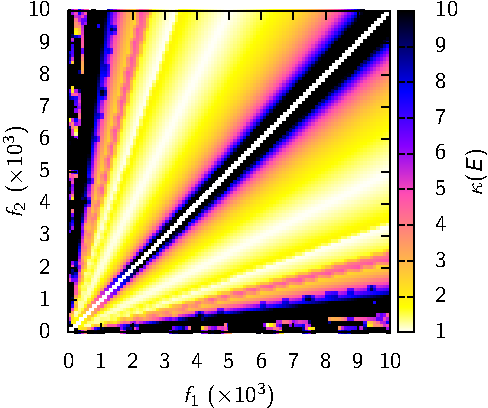
\includegraphics[width=.45\textwidth]{algo_apft_assessment.pdf}}
    \subfigure[OPT]{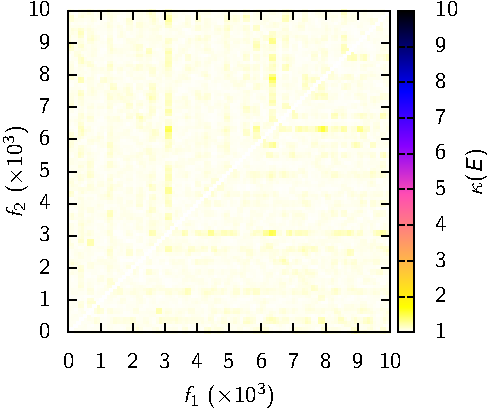
\includegraphics[width=.45\textwidth]{algo_opt_assessment.pdf}}
  \caption{Condition number of the discrete Fourier transform matrix $E$
  using two independent frequencies and four different algorithms
  to choose the time instances.}
  \label{fig:bench_algo}
\end{figure}

The EVE algorithms give fair results ($\kappa(E) \leq 2$) only at
discrete couples of frequencies, corresponding 
to the particular cases where $f_2$ is a
multiple of $f_1$, as shown in Sec.~\ref{sec:condition_cror_ael}. 
This is not promising as these
cases can be computed using the mono-frequential formulation and thus does not
need non-uniform time-instances. Oversampling improves the results. 
In fact, the mean condition number obtained
with $3N + 1$ samples indicates that the higher the number of time instances
the better the condition number. However the multi-frequential DFT
matrix becomes rectangular. The memory and CPU cost being proportional to 
the number of time instances (see Sec.~\ref{sec:sm_hb_cost}), 
such a strategy can not be
used in an industrial context. The APFT
algorithm improves the results, as it gives $\kappa (E) \leq 2$ 
for a large interval but fails when the frequencies
are too close from one another ($f_1 \approx f_2$) or when they are significantly
different ($f_1 \ll f_2$ or $f_1 \gg f_2$).  
Finally, the OPT algorithm gives a condition number close to unity for
all couple of frequencies $(f_1, f_2)$. Moreover, the OPT algorithm is
the only one to give a standard deviation that is smaller than the mean,
proving its robustness.
\begin{table}[htp]
  \ra{1.3} 
  \centering
  \begin{tabular}{lcccc}
    \toprule
    \phantom{abdefghijk} & min & max & mean & $\sigma$ \\
    \midrule
    EVE ($2N + 1$) & $1.0$ & $9.4\e{16}$ & $1.5\e{14}$ & $2.8\e{15}$ \\
    EVE ($3N + 1$) & $1.0$ & $3.7\e{16}$ & $4.7\e{13}$ & $9.5\e{14}$ \\
    APFT & $1.0$ & $81.2$ & $5.9$ & $9.0$ \\
    OPT & $1.0$ & $2.6$ & $1.1$ & $7.7\e{-2}$ \\
    \bottomrule
  \end{tabular}
  \caption{Condition number of the discrete Fourier transform matrix $E$
  statistics for two independent frequencies using four different algorithms
  to choose the time instances.}
  \label{tab:algo_sum}
\end{table} 

The configurations encountered in the turbomachinery literature 
are taken again to demonstrate the capability of the presented
algorithms to minimize the condition number
regardless of the input frequencies. The results are shown in 
Tab.~\ref{tab:literature_multistage2}.
The APFT algorithm improves the condition number compared to the
EVE ($2N+1$) but can give relatively large condition numbers, here $12.95$. 
In opposite, the OPT algorithm developed in the
present contribution gives results close to one for the four configurations.
\begin{table}[htp]
  \ra{1.3} \centering
  \begin{tabular}{rcccc}
    \toprule
    \multicolumn{1}{c}{Reference} & \multicolumn{4}{c}{$\kappa(E)$} \\
    \multicolumn{1}{c}{and \# harmonics} & EVE $(2N+1)$ & EVE $(3N+1)$ & APFT & OPT \\
    \midrule
    \citet{Gopinath2007} ($N=2$) & $\mathbf{3.79}$ & $3.00$ & $1.72$ & $1.08$ \\
    \citet{Ekici2007} ($N=3$) & $5.40$ & $\mathbf{3.84}$ & $1.71$ & $1.00$ \\
    \citet{Gopinath2007} ($N=4$) & $\mathbf{11.25}$ & $2.07$ & $3.46$ & $1.13$ \\
    \citet{Gopinath2007} ($N=7$) & $\mathbf{16.66}$ & $14.61$ & $12.95$ & $1.00$ \\
    \bottomrule
  \end{tabular}
  \caption{Literature review of the condition number used in multi-frequential
  harmonic balance computations compared to the presented algorithms.}
  \label{tab:literature_multistage2}
\end{table}

% Thus the proposed non-uniform time sampling combined with the OPT
% algorithm allows to tackle problems with large frequency
% separation. In such cases, the gain of the HB approach compared
% to classical time-marching methods is expected to be significant: with
% a time-marching scheme, the time-step has to be small enough to
% discretize the shortest period, while the number of time steps of the
% simulation has to be long enough to reach the steady-state
% (\emph{i.e.}  the simulation time is equal to several
% times the longest period). Conversely, as detailed in Sec.~\ref{sec:sm_hb_cost},
% the cost of the HB method only
% depends on the number of frequencies to capture, regardless of their
% relative values.

Thus, the non-uniform time sampling proposed by \citet{ThesisGuedeney}
used together with the OPT algorithm developed in the present contribution
enables to tackle problems with large frequency separation and/or large unsteadinesses,
namely CROR aeroelasticity.

\subsection{Distribution of the time instances}
For harmonically-related frequencies, the set of time instances
that minimize the condition number is 
provided by a uniform sampling of the fundamental frequency period
as it gives the theoretical lower bound $\kappa (E) = 1$. Since the
frequencies are harmonically related, the distribution of the time
instances on the other frequencies is also uniform. 
In fact, considering the
frequency vector $F = \left[f_1 \cdots f_k= kf_1 \cdots Nf_1 \right]$
and the time instances vector
$\mathbb{T}$ uniformly sampling the smallest frequency:
\begin{equation}
  \mathbb{T} = \left[0, \frac{1}{f_1 (2N+1)} \cdots  \frac{2N}{f_1 (2N+1)} \right],
  \label{eq:evenly_spaced_timelevels}
\end{equation}
then the product of the $i^{th}$ term of $\mathbb{T}$ to its
associated frequency is
\begin{equation}
  f_1 \frac{i}{f_1 (2N+1)} = k f_1 \frac{i}{k f_1 (2N+1)} = f_k \frac{i}{f_k (2N+1)}.
  \label{eq:evenly_spaced_timelevels_2}
\end{equation}
Equation~\eqref{eq:evenly_spaced_timelevels_2} means that evenly-spaced
time instances for the fundamental frequency are still seen as evenly
spaced by the $k^{th}$ harmonic. This is an explanation why the
condition number of the multi-frequential IDFT matrix $E^{-1}$ will be
unity as each frequency is sampled by evenly spaced time
instances~\cite{Brambilla1999}.

Now, considering non-harmonically related frequencies, there is
mathematically no reason for evenly-spaced time instances over the
smallest frequency to be seen as evenly spaced by the other frequencies
in general.

Figure~\ref{fig:distribution_tlv} shows the distribution of the time
instances, relative to each frequency period, obtained by the presented
algorithms for the frequencies $f_1 = 3$~Hz and $f_2 = 17$~Hz. 
To do so, the chosen time instances are redistributed
on the considered frequency period by applying a modulo to it:
\begin{equation}
  \label{eq:1}
  \mathbb{T}^{[f_k]}_j =  \mathbb{T}_j \text{ modulo } 1/f_k
\end{equation}
Then, they are divided by the latter, so that the results are
dimensionless.  In light gray line is depicted the $y=x$ function
representing the evenly-spaced solution on the considered period.
Keeping in mind that if each frequency sees evenly-spaced time instances,
then the condition number is the smallest, the optimal solution would
be to have relative time instances on $y=x$ for each period.  Running the
EVE $(2N + 1)$, APFT and OPT algorithms leads to a condition number of $33.1$,
$3.8$ and $1.1$, respectively.  The EVE algorithm gives a perfect distribution
of the time instances with respect to
period $1/f_1$ as the time instances are sampled on the period
$1/f_1$. However, it gives results that are far from the evenly spaced time instances
within period $1/f_2$. The APFT algorithm is nowhere near the evenly spaced
solution for both the considered periods, but closer than EVE regarding
period $1/f_2$. Finally, the OPT algorithm is the only one to be close
to the evenly spaced solution for each period considered. This explains the
very good condition numbers obtained with the OPT algorithm.
\begin{figure}[htp]
  \centering 
  \subfigure[relative to period $1/f_1$]{
      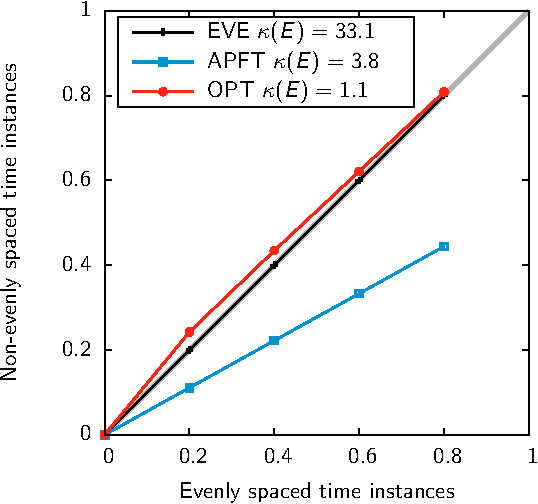
\includegraphics[width=.45\textwidth]{timelevels_distribution_f1.pdf}}
  \subfigure[relative to period $1/f_2$]{
      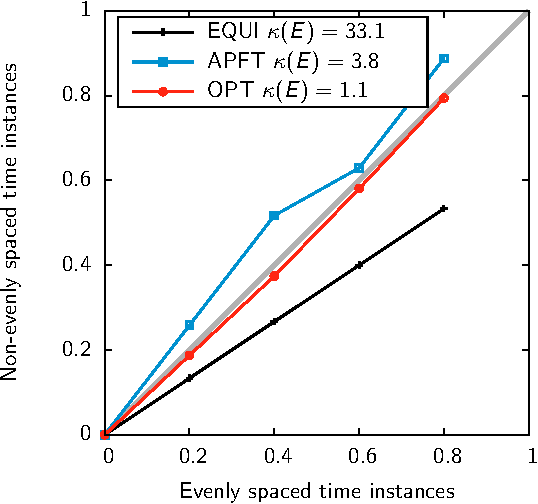
\includegraphics[width=.45\textwidth]{timelevels_distribution_f2.pdf}}
  \caption{Distribution of the time instances on each frequency periods.}
  \label{fig:distribution_tlv}
\end{figure}
